\documentclass[man,floatsintext]{apa6}
\usepackage{lmodern}
\usepackage{amssymb,amsmath}
\usepackage{ifxetex,ifluatex}
\usepackage{fixltx2e} % provides \textsubscript
\ifnum 0\ifxetex 1\fi\ifluatex 1\fi=0 % if pdftex
  \usepackage[T1]{fontenc}
  \usepackage[utf8]{inputenc}
\else % if luatex or xelatex
  \ifxetex
    \usepackage{mathspec}
  \else
    \usepackage{fontspec}
  \fi
  \defaultfontfeatures{Ligatures=TeX,Scale=MatchLowercase}
\fi
% use upquote if available, for straight quotes in verbatim environments
\IfFileExists{upquote.sty}{\usepackage{upquote}}{}
% use microtype if available
\IfFileExists{microtype.sty}{%
\usepackage{microtype}
\UseMicrotypeSet[protrusion]{basicmath} % disable protrusion for tt fonts
}{}
\usepackage{hyperref}
\hypersetup{unicode=true,
            pdftitle={Reminder about Confidence Intervals},
            pdfauthor={Marie Delacre},
            pdfkeywords={keywords},
            pdfborder={0 0 0},
            breaklinks=true}
\urlstyle{same}  % don't use monospace font for urls
\usepackage{graphicx,grffile}
\makeatletter
\def\maxwidth{\ifdim\Gin@nat@width>\linewidth\linewidth\else\Gin@nat@width\fi}
\def\maxheight{\ifdim\Gin@nat@height>\textheight\textheight\else\Gin@nat@height\fi}
\makeatother
% Scale images if necessary, so that they will not overflow the page
% margins by default, and it is still possible to overwrite the defaults
% using explicit options in \includegraphics[width, height, ...]{}
\setkeys{Gin}{width=\maxwidth,height=\maxheight,keepaspectratio}
\IfFileExists{parskip.sty}{%
\usepackage{parskip}
}{% else
\setlength{\parindent}{0pt}
\setlength{\parskip}{6pt plus 2pt minus 1pt}
}
\setlength{\emergencystretch}{3em}  % prevent overfull lines
\providecommand{\tightlist}{%
  \setlength{\itemsep}{0pt}\setlength{\parskip}{0pt}}
\setcounter{secnumdepth}{0}
% Redefines (sub)paragraphs to behave more like sections
\ifx\paragraph\undefined\else
\let\oldparagraph\paragraph
\renewcommand{\paragraph}[1]{\oldparagraph{#1}\mbox{}}
\fi
\ifx\subparagraph\undefined\else
\let\oldsubparagraph\subparagraph
\renewcommand{\subparagraph}[1]{\oldsubparagraph{#1}\mbox{}}
\fi

%%% Use protect on footnotes to avoid problems with footnotes in titles
\let\rmarkdownfootnote\footnote%
\def\footnote{\protect\rmarkdownfootnote}


  \title{Reminder about Confidence Intervals}
    \author{Marie Delacre\textsuperscript{1}}
    \date{}
  
\shorttitle{CI REMINDER}
\affiliation{
\vspace{0.5cm}
\textsuperscript{1} ULB}
\keywords{keywords\newline\indent Word count: X}
\usepackage{csquotes}
\usepackage{upgreek}
\captionsetup{font=singlespacing,justification=justified}

\usepackage{longtable}
\usepackage{lscape}
\usepackage{multirow}
\usepackage{tabularx}
\usepackage[flushleft]{threeparttable}
\usepackage{threeparttablex}

\newenvironment{lltable}{\begin{landscape}\begin{center}\begin{ThreePartTable}}{\end{ThreePartTable}\end{center}\end{landscape}}

\makeatletter
\newcommand\LastLTentrywidth{1em}
\newlength\longtablewidth
\setlength{\longtablewidth}{1in}
\newcommand{\getlongtablewidth}{\begingroup \ifcsname LT@\roman{LT@tables}\endcsname \global\longtablewidth=0pt \renewcommand{\LT@entry}[2]{\global\advance\longtablewidth by ##2\relax\gdef\LastLTentrywidth{##2}}\@nameuse{LT@\roman{LT@tables}} \fi \endgroup}


\usepackage{lineno}

\linenumbers

\authornote{

Correspondence concerning this article should be addressed to Marie Delacre, Postal address. E-mail: \href{mailto:marie.delacre@ulb.ac.be}{\nolinkurl{marie.delacre@ulb.ac.be}}}

\abstract{

}

\begin{document}
\maketitle

\hypertarget{reference}{%
\subsection{Reference}\label{reference}}

Cumming, G., \& Finch, S. (2001). A primer on the understanding, use, and calculation of confidence intervales that are based on central and noncentral distributions. Educational and Psychological Measurement, 61(532).

\hypertarget{how-to-determine-the-ci-around-a-parameter}{%
\section{How to determine the CI around a parameter}\label{how-to-determine-the-ci-around-a-parameter}}

\hypertarget{method-1-method-based-on-the-use-of-a-pivotal-quantity}{%
\subsection{Method 1: method based on the use of a pivotal quantity}\label{method-1-method-based-on-the-use-of-a-pivotal-quantity}}

When computing a (supposed normal) centered variable, divided by the standard error (i.e.~an independant variable closely related with the \(\chi^2\) distribution), then computed quantity will follow a central \emph{t}-distribution. This quantity is called a pivotal quantity (PQ), i.e.~a quantity that is very interesting because its sampling distribution is not a function of the parameter we want to estimate (Cox \& Hinkley, 1974 cited by Cumming and Finch, 2001). We can therefore use it, in order to define confidence limits for any parameter.

The method consists in four steps:\\
1) Compute a pivotal quantity (PQ) of the general form: (Estimator - parameter)/SE;\\
2) Determining the distribution of PQ;\\
3) Computing the confidence limits of PQ: determine a range of values, centered around 0, such as (1-alpha)\% of the area under the distribution of PQ falls in this range;\\
4) Pivote in order to obtain the confidence interval around the parameter of interest.

As a first example, consider the case of 2 means difference, assuming normality and homoscedasticity. The pivotal quantity is defined as follows:

\begin{equation} 
PQ= \frac{(\bar{X_1}-\bar{X_2})-(\mu_1-\mu_2)}{SE}
\label{eq:PQstudent}
\end{equation}

With \(SE = \sigma_{pooled} \times \sqrt{\frac{1}{n_1}+\frac{1}{n_2}}\) and \(\sigma_{pooled} = \sqrt{\frac{(n_1-1)*S^2_1+(n_2-1)*S^2_2}{n_1+n_2-2}}\)

This quantity follows a \emph{t}- distribution with \(n_1+n_2-2\) degrees of freedom (therefore, it depends only on \(n_1\) and \(n_2\), it does NOT depend on the parameter of interest, i.e.~\(\mu_1-\mu_2\)).

\begin{figure}
\centering
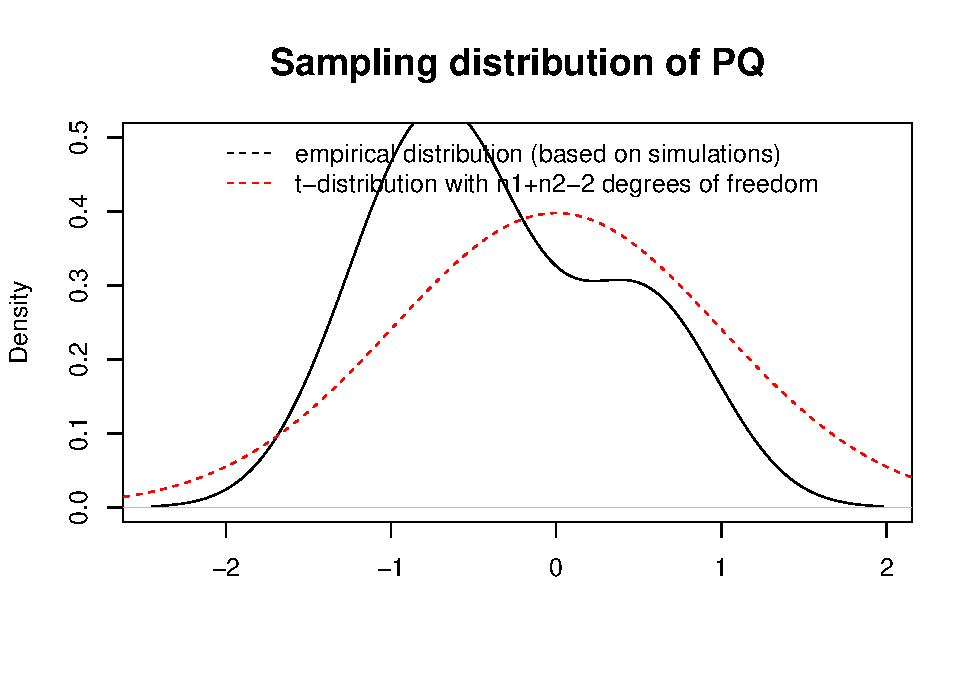
\includegraphics{CI-Reminder_files/figure-latex/SAMPLMEANDIFF1-1.pdf}
\caption{\label{fig:SAMPLMEANDIFF1}Sampling distribution of the pivotal quantity under the assumptions of normality and homoscedasticity}
\end{figure}

Because the theoretical distribution of PQ is known, one can compute the confidence limits, for any confidence level:

\begin{equation} 
Pr[t_{n_1+n_2-2}(\frac{\alpha}{2}) < \frac{(\bar{X_1}-\bar{X_2})-(\mu_1-\mu_2)}{SE} < t_{n_1+n_2-2}(1-\frac{\alpha}{2})] = 1 - \alpha
\label{eq:conflev1}
\end{equation}

Because the \emph{t}-distribution is symmetrically centered around 0, one can deduce that \(t_{n_1+n_2-2}(\frac{\alpha}{2})=-t_{n_1+n_2-2}(1-\frac{\alpha}{2})\), and therefore:

\begin{equation} 
Pr[-t_{n_1+n_2-2}(1-\frac{\alpha}{2}) < \frac{(\bar{X_1}-\bar{X_2})-(\mu_1-\mu_2)}{SE} < t_{n_1+n_2-2}(1-\frac{\alpha}{2})] = 1 - \alpha
\label{eq:conflev2}
\end{equation}

In pivoting the inequation, one can deduce that:

\begin{equation} 
Pr[-t_{n_1+n_2-2}(1-\frac{\alpha}{2}) \times SE < (\bar{X_1}-\bar{X_2})-(\mu_1-\mu_2) < t_{n_1+n_2-2}(1-\frac{\alpha}{2}) \times SE] = 1-\alpha
\label{eq:conflev3}
\end{equation}

\begin{equation} 
\leftrightarrow Pr[-(\bar{X_1}-\bar{X_2}) -t_{n_1+n_2-2}(1-\frac{\alpha}{2}) \times SE <
-(\mu_1-\mu_2) 
< -(\bar{X_1}-\bar{X_2}) +t_{n_1+n_2-2}(1-\frac{\alpha}{2}) \times SE]= 1- \alpha
\label{eq:conflev4}
\end{equation}

\begin{equation} 
\leftrightarrow Pr[(\bar{X_1}-\bar{X_2}) +t_{n_1+n_2-2}(1-\frac{\alpha}{2}) \times SE > \mu_1-\mu_2 > (\bar{X_1}-\bar{X_2}) - t_{n_1+n_2-2}(1-\frac{\alpha}{2}) \times SE]= 1- \alpha
\label{eq:conflev5}
\end{equation}

\begin{equation} 
\leftrightarrow Pr[(\bar{X_1}-\bar{X_2}) - t_{n_1+n_2-2}(1-\frac{\alpha}{2}) \times SE < \mu_1-\mu_2 <(\bar{X_1}-\bar{X_2}) +t_{n_1+n_2-2}(1-\frac{\alpha}{2}) \times SE]= 1- \alpha
\label{eq:conflev6}
\end{equation}

As a second example, consider the case of 2 means difference, assuming normality and heteroscedasticity. The pivotal quantity is defined as follows:

\begin{equation} 
PQ= \frac{(\bar{X_1}-\bar{X_2})-(\mu_1-\mu_2)}{SE}
\label{eq:PQwelch}
\end{equation}

With \(SE = \sqrt{\frac{S^2_1}{n1}+\frac{S^2_2}{n2}}\)

This quantity follows a \emph{t}- distribution with \(\frac{(\frac{S^2_1}{n_1}+\frac{S^2_2}{n_2})^2}{\frac{(\frac{S^2_1}{n_1})^2}{n_1-1}+\frac{(\frac{S^2_2}{n_2})^2}{n_2-1}}\) degrees of freedom (therefore, it depends on \(n_1\) and \(n_2\), \(S_1\) and \(S_2\), and does NOT depend on the parameter of interest, i.e.~\(\mu_1-\mu_2\)).

\begin{figure}
\centering
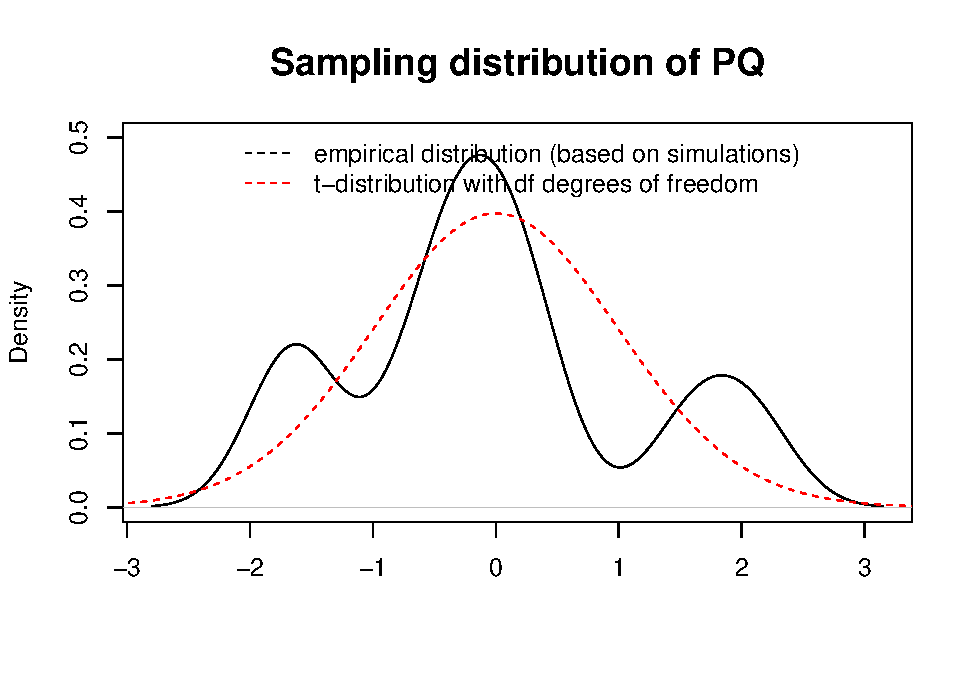
\includegraphics{CI-Reminder_files/figure-latex/SAMPLMEANDIFF2-1.pdf}
\caption{\label{fig:SAMPLMEANDIFF2}Sampling distribution of the pivotal quantity under the assumptions of normality and heteroscedasticity}
\end{figure}

Because the theoretical distribution of PQ is known, one can compute the confidence limits, for any confidence level (see the first example for more details):

\begin{equation} 
Pr[(\bar{X_1}-\bar{X_2}) - t_{n_1+n_2-2}(1-\frac{\alpha}{2}) \times SE < \mu_1-\mu_2 <(\bar{X_1}-\bar{X_2}) +t_{n_1+n_2-2}(1-\frac{\alpha}{2}) \times SE]= 1- \alpha
\label{eq:conflev6}
\end{equation}

With SE = \(\sqrt{\frac{S_1^2}{n_1}+\frac{S_2^2}{n_2}}\)

\hypertarget{method-2}{%
\subsection{Method 2}\label{method-2}}

We can also think of confidence limits as the most extreme values of \(\mu_1-\mu_2\) that we could define as null hypothesis and that would not lead to rejecting the null hypothesis. In other words, we could define the lower limit such as \(\bar{X_1}-\bar{X_2}\) exactly equals the quantile (1-\(\frac{\alpha}{2}\)) of the central \emph{t}-distribution of the null hypothesis \(H_0: \mu_1 - \mu_2 = (\mu_1-\mu_2)_L\), and the upper limit such as \(\bar{X_1}-\bar{X_2}\) exactly equals the quantile \(\frac{\alpha}{2}\) of the central \emph{t}-distribution of the null hypothesis \(H_0: \mu_1 - \mu_2 = (\mu_1-\mu_2)_U\):

\begin{equation} 
Pr[t_{n_1+n_2-2} >= \frac{(\bar{X_1}-\bar{X_2})-(\mu_1-\mu_2)_L}{SE}]= 1- \alpha
\label{eq:plausiblelimit1}
\end{equation}

\begin{equation} 
Pr[t_{n_1+n_2-2} <= \frac{(\bar{X_1}-\bar{X_2})-(\mu_1-\mu_2)_U}{SE}]= 1- \alpha
\label{eq:plausiblelimit2}
\end{equation}

This concept of the problem helps to understand how we calculate the confidence intervals around the effect size measures, as explained below.

\hypertarget{how-to-determine-the-ci-around-cohens-delta}{%
\section{\texorpdfstring{How to determine the CI around Cohen's \(\delta\)}{How to determine the CI around Cohen's \textbackslash delta}}\label{how-to-determine-the-ci-around-cohens-delta}}

\begin{figure}
\centering
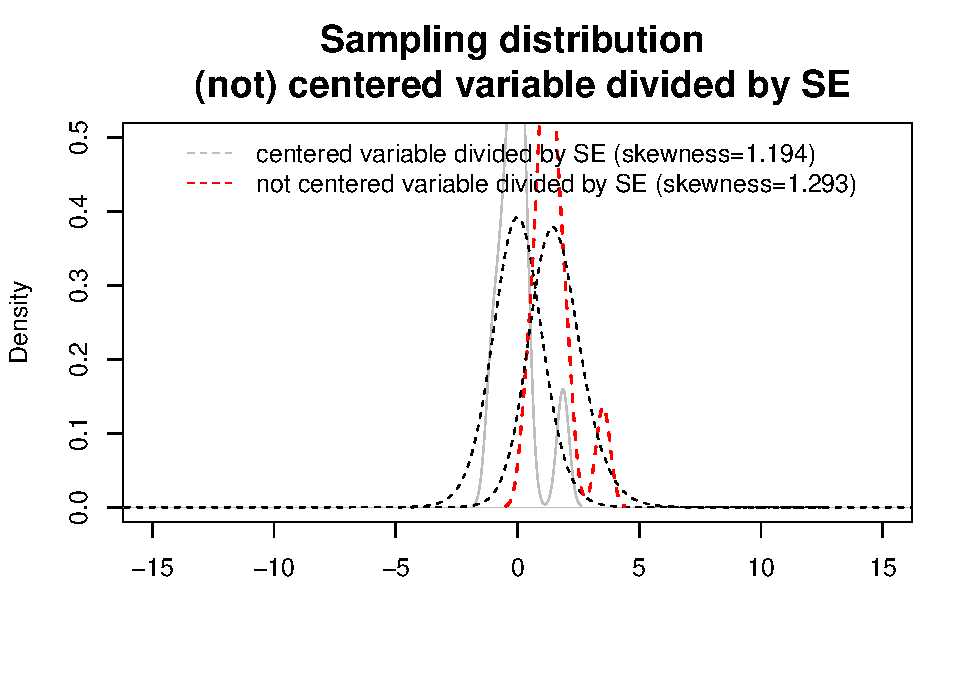
\includegraphics{CI-Reminder_files/figure-latex/SAMPLMEANDIFF3-1.pdf}
\caption{\label{fig:SAMPLMEANDIFF3}Sampling distribution of centered mean difference divided by SE (in grey, i.e.~pivotal quantity) and not centered mean difference divided by SE (in red), assuming normality and homoscedasticity.}
\end{figure}

Consider the following quantity:
\begin{equation} 
t_{obs}=\frac{(\bar{X_1}-\bar{X_2})-(\mu_1-\mu_2)_0}{SE}
\label{eq:plausiblelimit2}
\end{equation}

With \(SE = \sigma_{pooled} \times \sqrt{\frac{1}{n_1}+\frac{1}{n_2}}\) and \(\sigma_{pooled} = \sqrt{\frac{(n_1-1)*S^2_1+(n_2-1)*S^2_2}{n_1+n_2-2}}\), and \((\mu_1-\mu_2)_0\) is the means difference under the null hypothesis. If the null hypothesis is true, this quantity is a (supposed normal) centered variable, divided by an independant variable closely related with the \(\chi^2\). Therefore, as previously mentioned, it will follow a central \emph{t}-distribution. However, if the null hypothesis is false, the distribution of this quantity will not be centered, and Noncentral \emph{t}-distribution will arise, as illustrated in Figure \ref{fig:SAMPLMEANDIFF3} for the case of 2 means difference, assuming normality and homoscedasticity.

Noncentral \emph{t}-distributions are described by two parameters: degrees of freedom (df) and noncentrality parameter (that we will call \(\lambda\)). \(\lambda\) is a function of \(\delta\) and sample sizes:

\begin{equation}
\lambda = \frac{\mu_1-\mu_2}{\sigma_{pooled}} \times \sqrt{\frac{n_1 \times n_2}{n_1 + n_2}}
\label{eq:ncp}
\end{equation}

Like we did in second method to determine a confidence interval around the mean difference, we could try to determine the \emph{t}-distributions for which \(t_{obs}\) corresponds respectively to the \(1-\frac{\alpha}{2}\) and to the \(\frac{\alpha}{2}\) th. quantile. Because we know that degrees of freedom will equal \(n_1+n_2-2\), the unknown parameter of the \emph{t}-distributions to be determined is \(\lambda\). In other word, we should determine the non centrality parameter (\(\lambda_L\)) of distributions such as \[P[t_{n_1+n_2-2, \lambda} >= t_{obs}] = 1- \alpha \] and the non centrality parameter (\(\lambda_U\)) of distributions such as \[P[t_{n_1+n_2-2, \lambda} <= t_{obs}] = 1- \alpha \]. One we have defined confidence limits for \(\lambda\), one can divide them by \(\sqrt{\frac{n_1 \times n_2}{n_1 + n_2}}\) in order to have confidence limits for \(\delta\).


\end{document}
